\title{Two Example Review Problems from Group Session}
\author{Jordan Hanson}
\date{\today}

\documentclass[12pt]{article}
\usepackage{amsmath}
\usepackage{graphicx}

\begin{document}
\maketitle

\begin{abstract}
We finished all but two example problems today in lecture.  The following two refer to concepts from uniform circular motion.
\end{abstract}

\section{Motorcycle Circus}

\textit{First example of this type of problem}: \\
Suppose a motorcycle is riding at a speed $v$ inside a sphere with coefficient of static friction $\mu_{\rm s}$, and the speed is high enough such that the motorcycle is traveling around the equator of the sphere, horizontally.  In this example, static friction acts in the upward direction, and gravity acts in the downward direction.  The net force, therefore, in the vertical axis is
\begin{equation}
\vec{F}_{\rm net} \cdot \hat{j} = \vec{F}_{\rm net,y} = \vec{f}_{\rm f,s} - \vec{w} = 0
\label{eq:eq1}
\end{equation}
Eq. \ref{eq:eq1} yields
\begin{equation}
f_{\rm f,s} = w
\end{equation}
In the plane containing the equator of the sphere, there are two forces: centripetal and normal.  By running the engine, the motorcycle goes in a straight line, but the curvature of the sphere turns the bike inward.  Thus, the normal force \textit{supplies} or \textit{provides} the centripetal force
\begin{equation}
\vec{F}_{\rm net} \cdot \hat{i} = \vec{F}_{\rm net,x} = f_{\rm C} = N
\label{eq:eq2}
\end{equation}
Let $m$ be the mass of the bike, and $r$ be the radius of the sphere.  The magnitude of the normal force is given by
\begin{equation}
f_{\rm C} = mv^2/r
\end{equation}
And so
\begin{equation}
N = mv^2/r
\end{equation}
However,
\begin{equation}
f_{\rm f,s} = \mu_{\rm s} N = \mu_{\rm s} mv^2/r
\end{equation}
Since friction balances gravity in the vertical direction,
\begin{align}
\mu_{\rm s} mv^2/r &= mg \\
v &= \sqrt{\frac{rg}{\mu_{\rm s}}}
\end{align}
The velocity has to be high enough such that the ensuing normal force cancels gravity by the associated normal force.  Put another way, if the velocity is too low, the friction (through the normal force) will be too little to keep the bike from sliding down the side.  (Note: the rider must also lean upwards away from the direction of gravity to cancel the \textbf{torque}, since the force of gravity acts on the center of mass of the bike system).\\ \\
\textit{Second example of this type of problem}: \\
Now suppose the bike is not traveling around the equator of the sphere, but the \textit{meridian} of the sphere.  Suppose that the speed constant $v$ is given, and that it is high enough for the bike to make the loop.  Also let there be friction between the bike wheels and the sphere, and the mass of the bike be $m$.  The goal is to calculate the normal force and the force of friction when the bike is at the bottom of the sphere ($\theta = 0$), the side while going up ($\theta = \pi/2$), the top ($\theta = \pi$), and 45 degrees past the top ($\theta = 5\pi/4$).
\begin{itemize}
\item \textbf{At the bottom}: The centripetal force is constant because the speed is constant.  It must be the net force in the vertical direction.  The weight from gravity points down, and the normal force points up:
\begin{align}
N - mg &= \frac{mv^2}{r} \\
N &= m\left(\frac{v^2}{r}+g\right)
\end{align}
The frictional force is zero, since it is static friction but there is no acceleration in the horizontal direction.
\item \textbf{At $\theta = \pi/2$}:  There are now forces in the horizontal and vertical directions.  The vertical net force is zero, because there is no accleration in the vertical direction.  Therefore weight must be balanced by static friction:
\begin{equation}
f_{\rm f,s} = w
\end{equation}
If the tires had no traction (that is, no static friction), then the bike would merely slide down the side of the sphere.  In the horizontal direction, the centripetal force is supplied by the normal force:
\begin{equation}
N = mv^2/r
\end{equation}
\item \textbf{At the top}: There are no horizontal forces at $\theta = \pi$, because the velocity is constant and the gravity and normal forces point down.  The centripetal force is the net force, and it points down as well, so
\begin{align}
-mg - N &= -mv^2/r \\
N &= m\left(\frac{v^2}{r} - g\right)
\end{align}
The normal force is less strong than at the bottom ($\theta = 0$), because gravity is pulling down on the bike.
\item \textbf{At $\theta = 5\pi/4$}: The situation is similar to the incline plane class of problems, where the gravity vector must be broken into two components: the component anti-parallel to the motion ($mg\sin\phi$), and the component normal to the surface ($mg\cos\phi$), for $\phi = \pi/4$, or 45 degrees past vertical.  For the forces normal to the sphere surface:
\begin{align}
N + mg\cos\phi = mv^2/r& \\
N = m\left(\frac{v^2}{r}-g\cos\phi \right)
\end{align}
The normal force is less than at the sides of the sphere, but more than at the top.  For the parallel forces:
\begin{equation}
f_{\rm f,s} = mg\sin\theta
\end{equation}
If the static friction did not cancel the parallel component of gravity, the bike would slide down the side of the sphere.
\end{itemize}

\section{Discrete Angular Motion of a Particle Becoming Uniform Circular Motion}

\begin{figure}
\centering
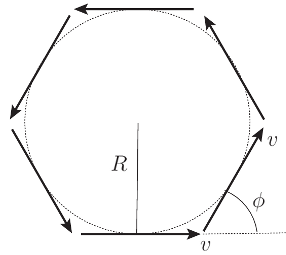
\includegraphics[width=0.4\textwidth]{circle.png}
\caption{\label{fig:fig1} A particle moves (on average) in circular uniform motion.}
\end{figure}

A particle moves according to Fig. \ref{fig:fig1}.  During a time interval $\Delta t$, the velocity of the particle changes by an angle $\phi$.  The initial velocity is $\vec{v}_{\rm i} = v\hat{i}$.  The final velocity is $\vec{v}_{\rm f} = v\cos\phi \hat{i} + v\sin\phi \hat{j}$.  The average acceleration is
\begin{equation}
\bar{a} = \frac{\vec{v}_{\rm f} - \vec{v}_{\rm i}}{\Delta t} = v\frac{(\cos\phi - 1) \hat{i} + \sin\phi \hat{j}}{\Delta t}
\end{equation}
Although the polygon shown in Fig. \ref{fig:fig1} is six-sided with $\phi=60$ degrees, increasing the number of sides more and more decreases $\phi$.  \textbf{The key concept for this problem is that a larger number of sides makes the motion more and more circular, and $\phi\ll1$}.  For $\phi\ll 1$,
\begin{equation}
\lim_{\phi \to 0} \bar{a} = v\frac{(1 - \phi^2/2 - 1) \hat{i} + \phi \hat{j}}{\Delta t} \approx v\frac{\phi \hat{j}}{\Delta t}
\label{eq:eq3}
\end{equation}
It might seem puzzling that the acceleration is getting close to zero because $\phi$ is so small as the number of sides grows.  It can be shown geometrically that $\phi = 2\pi/N$, so Eq. \ref{eq:eq2} is like taking the limit
\begin{equation}
\lim_{N \to \infty} \bar{a} = v\frac{2\pi\hat{j}}{N\Delta t}
\label{eq:eq4}
\end{equation}
However, $2\pi/N\Delta t = 2\pi/T$, where $T$ is the period, because it is $N$ steps of $\Delta t$ all the way around the polygon.  Notice that $2\pi/T = 2\pi f$, where $f$ is the period, and finally, $2\pi f = \omega$.  Thus,
\begin{equation}
\lim_{N \to \infty} \bar{a} = v\omega
\label{eq:eq5}
\end{equation}
But we know that in this limit ($\Delta t \to 0$, $N \to \infty$) that $\omega = v/r$.  Subsituting $v/r$ for $\omega$ in Eq. \ref{eq:eq5} yields
\begin{equation}
\lim_{N \to \infty} \bar{a} = \frac{v^2}{r}\hat{j}
\label{eq:eq6}
\end{equation}
Equation \ref{eq:eq6} reveals that the centripetal acceleration is
\begin{equation}
\vec{a}_{\rm C} = \frac{v^2}{r} \hat{j}
\end{equation}
From Fig. \ref{fig:fig1}, the angle $\phi$ is defined such that $\hat{j}$ points towards the center of the circle.  In general, if the unit vector $-\hat{r}$ points to the center, the final conclusion is that
\begin{equation}
\boxed{\vec{a}_{\rm C} = -\frac{v^2}{r}\hat{r}}
\end{equation}
\end{document}